\section{Abstract Argumentation}
\label{sec: abstract-argumentation}

This section is devoted to the \textit{abstract argumentation theory} \zh{抽象论辩理论} introduced in the seminal paper \cite{Dun1995} by  Dung.
% 
This formalism is based on the idea that arguments are defeasible entities which may attack each other and whose acceptance is subject to a given reasonable criterion (called \textit{semantics}).
% 
Formally, 
an argumentation framework is represented as a directed graph in which the arguments are represented as nodes and the attack relations as  edges.
% 


Given such a graph, 
a key question is which set(s) of arguments can be accepted.
That is, 
once the argumentation framework has been constructed, 
how to determine which arguments to accept or reject?
% 
To answer this kind of questions corresponding to define an \textit{argumentation semantics} \zh{论辩语义}.
%
% 
By and large, 
two kinds of approaches for argumentation semantics are available in the literature: 
\begin{enumerate}[itemsep=5pt,parsep=0pt,leftmargin=3em,topsep=5pt,label=(\arabic*)]
    \item the \textit{extension}--based approach \zh{基于外延的方法}, proposed in Dung's original paper \cite{Dun1995}, and
    \item the \textit{labelling}--based approach \zh{基于标签的方法}.
\end{enumerate}
% 
In this note, 
however, 
for the sake of simplicity,
we only focus on the first one.
% , let alone the correspondence between those two approaches.





% Dung's theory can be regarded as an attack/conflict calculus, 
% which has been initially formulated for the need of dealing with attacks between arguments but then stands on its own feet, 
% even independently of the original interpretation in argumentative terms.



% applications: 
% \begin{itemize}[itemsep=5pt,parsep=5pt,leftmargin=3em,topsep=5pt]
%     \item inference from a knowledge base
%     \item decision--making
%     \item coalition formation
%     \item stable marriage problem
%     \item argument-based reasoning
% \end{itemize}


% When an argumentation framework was given,
% it is then interesting to identify the \textit{conflict-free outcomes}, 
% which, roughly speaking, 
% means determining which arguments should be accepted (let's say, ``survive the conflict'') and which arguments should be rejected (let's say, ``are defeated in the conflict''), 
% according to some reasonable criterion.
% % 
% A formal method to identify those outcomes for any argumentation framework is called \textit{argumentation semantics}.
% 
% 



\begin{comment}

The idea underlying the \textit{labelling}-based approach is to give each argument a label. 
A sensible (though not the only possible) choice for the set of labels is $\Lambda = \{\mathsf{in}, \mathsf{out}, \mathsf{undec}\}$,
where the label \textsf{in} means the argument is accepted, 
the label \textsf{out} means the argument is rejected and the label \textsf{undec} means one abstains from an opinion on whether the argument is accepted or rejected. 
Each argument then gets exactly one label.

A specific labelling-based argumentation semantics provides a way to select “reasonable” labellings among all the possible ones, 
according to some criterion embedded in its definition.


A first investigation of the connections between defeat status assignments and extensions in Dung's argumentation frameworks was provided in \cite{Verheij1996}.

\dotfill
\vspace{1.5em}
\end{comment}








% Some preliminaries and notation: 
% arguments in any argumentation framework will be denoted by lowercase Latin letters: $a,b,c, \dots$.






% central notion: acceptability of arguments.





% \textit{The one who has the last word laughs best}.



% \vspace{3em}



% Roughly, 
% the idea of argumentational reasoning is that a statement is believable if it can be argued successfully against attacking arguments. 
% In other words, 
% whether or not a rational agent believes in a statement depends on whether or not the argument supporting this statement can be successfully defended against the counterarguments. 



% \vspace{3em}


%  argumentation  can be viewed as logic programming with negation as failure.
% % 
% This result shows that logic programming is the perfect tool for implementing argumentation systems.


% \vspace{3em}




% /////////////////////////////////////////////////////////////////////////////
\subsection{Abstract Argumentation frameworks}
\label{subsec: abstract-argumentation-frameworks}


An (abstract) argumentation framework is nothing, 
mathematically speaking, 
but a pair consists of a set of arguments and a binary relation representing the attack relationship between arguments, 
that is, 
a \textit{directed graph} in which the arguments as nodes and the attack relations as arrows. 
% 
An argument is an abstract entity whose role is solely determined by its relations to other arguments.



\begin{df}[Argumentation frameworks, AFs]
    An \textit{argumentation framework} \zh{论辩框架} is a pair 
    \[
        {\color{purple} AF = (Arg,\att)}
    \]
    where $Arg$ is a non--empty set of arguments, 
    and $\att \;\subseteq Arg \times Arg$ is a binary relation on $Ar$.
\end{df}



Given an AF $AF=(Arg,\att)$, 
let $a,b \in Arg$, 
we say that $a$ \textit{attacks/defeats} $b$ (accordingly, $a$ is an \textit{attacker} of $b$) iff $a \att b$ holds.
% 
For any $X \cup \{a\} \subseteq Arg$, 
then we say that $X$ \textit{attacks} $a$, 
denoted as {\color{purple} $X \att a$}, 
if there exists $b \in X$ s.t. $b \att a$.
% 
Likewise, 
we say that $a$ \textit{attacks} $X$, 
written as {\color{purple} $a \att X$}, 
if there is $b \in X$ s.t. $a \att b$.
% 
For $a \in Arg$, 
we define the sets $a^-$ and $a^+$ as follows: \zh{各种攻击关系}
\[
\begin{array}{rll}
    {\color{purple} a^-} &\coloneqq& \{b \in Arg \mid b \att a\},  \\
    
    {\color{purple} a^+} &\coloneqq& \{b \in Arg \mid a \att b\}.  \\
\end{array}
\]
Those two operations can be extended att any subset $X \subseteq Arg$ by
\[
    {\color{purple} X^\pm}   = \bigcup_{a \in X} a^\pm 
    \qquad
    \pm \in\{+,-\}.
\]



The attack relations between argument(s) aforementioned are summarized in Table~\ref{tab: attack-relation}. 
% In what follows, 
% we will use $\not\att$ to denote the negation of $\att$.

% attack relationships
\begin{table}[ht!]
    \centering
    \caption{The attack relations between argument(s)}
    \label{tab: attack-relation} 
    \renewcommand{\arraystretch}{1.2}
    \begin{tabular}{l||ll}
    \hline
    \multicolumn{1}{c||}{notation} & 
    \multicolumn{1}{c}{meaning} \\
    \hline

    $a \att b$ & 
    $a$ attacks $b$  \\

    $a \att X$ &  
    $a$ attacks $X$ ($\exists b \in X: a \att b$) \\ 

    $X \att a$  &  
    $X$ attacks $a$  ($\exists b \in X: b \att a$) \\

    
    $X \att Y$ &
    $X$ attacks $Y$ 
    ($\exists a \in X, \exists b \in Y: a \att b$)  \\

    \hline
\end{tabular}
\end{table}






% \begin{df}[Subframes]
%     Given an AF $\mathcal{AF} = (Ar,\to)$ and a set of arguments $X \subseteq Ar$, 
%     the restriction of $\mathcal{AF}$ to $X$, 
%     denoted as $\mathcal{AF}_X$, 
%     is the argumentation framework $(X,\to_X)$ where 
%     $\to_X \;=\; \to \cap (X\times X)$.    
% \end{df}


% \vspace{3em}
% Doing abstract argumentation theory means, essentially, 
% to study specific properties of subsets of the set of arguments in a given argumentation framework.




% /////////////////////////////////////////////////////////////////////////////
% \subsection{Argumentation Semantics (extension-based)}
% \subsection{Argumentation Semantics}
% \label{subsec: basic-definition}



% \vspace{1.5em}

% a simple principle: 
% for every argument $a$ one accepts or rejects one should be able to explain why it is accepted or rejected, 
% taking into account the acceptance or rejection of other arguments connected to $a$ through the attack relation. 



\begin{df}[Defense]
    Let $AF=(Arg,\att)$ be an AF and $X \subseteq Arg$. 
    % 
    The set $X$ \textit{defends} $a \in Arg$ 
    (or, ``$a$ \textit{acceptable} w.r.t. $X$''\footnote{
    This is the original terminology in Dung's paper \cite{Dun1995}.
    }) 
    iff 
    $\forall b \in Arg:b \att a \Rightarrow X \att b$
    (or equivalently, $\forall b \in a^- : X \att b$, 
    where $a^-$ is the set of attackers of $a$). 
    \zh{辩护}
\end{df}




According to vacuous truth,
if $a^- = \emptyset$
(such $a$ are called \textit{initial arguments}, 
the set of initial arguments of an $AF$ denoted as {\color{purple} $\mathcal{NI}(AF)$}, i.e., 
$\mathcal{IN}(AF) =  \{a \in Ar \mid a^- = \emptyset\}$)
then $a$ defended by any set of arguments, 
including $\emptyset$ of course.




\begin{df}[Characteristic function]
    Let $AF=(Arg,\att)$ be an AF. 
    % 
    The \textit{characteristic function} of $AF$ is mapping 
    $C_{AF} \colon \wp(Arg) \to \wp(Arg)$ such that 
    \[
        C_{AF} (X) 
            = 
        \{a \in Arg \mid X \text{~defends~} a\}
    \]
    for each $X \subseteq Arg$.       \zh{刻画函数}
\end{df}

% In what follows, 
% for the sake of brevity,
% we will simply notate $C_{AF}$ as $C$ if no confusion arises.


\begin{prop} 
    For any AF $AF=(Arg,\att)$, 
    then:
    \begin{enumerate}[itemsep=5pt,parsep=5pt,leftmargin=3em,topsep=5pt,label=(\arabic*)] %% or label = \alph*, \roman*
        \item 
        $C_{AF}(\emptyset)=\mathcal{IN}(AF)=\{a \in Arg \mid a^- = \emptyset\}$.
        

        \item 
        $\mathcal{IN}(AF) \subseteq C_{AF}(X)$.


        \item $C_{AF}(X) = (X^+)^+$.
        % [AC98] L. Amgoud and C. Cayrol. On the acceptability of arguments in preference-based argumentation. In G. Cooper and S. Moral, editors, Proceedings of the 14th Conference on Uncertainty in Artificial Intelligence (UAI 1998), pages 1–7. Morgan Kaufmann, 1998.
    \end{enumerate}
    where $X \subseteq Arg$.
\end{prop}




\begin{df}[Conflict--freeness]
    Let $AF=(Arg,\att)$ be an AF and $X \subseteq Arg$.
    % 
    $X$ is said to be  \textit{conflict--free} \zh{无冲突} iff 
    $\neg\exists a,b \in X: a \att b$.  
\end{df}



Clearly, 
the emptyset $\emptyset$ is conflict--free.
%
Furthermore,  
if each argument has at least one attacker, 
i.e. $a^- \not=\emptyset$ for every argument $a$, 
then  $\emptyset$ is a (conflict--free) fixed point of the characteristic function.
\zh{什么情况下空集是不动点}




After introduced the notion of \textit{defense}, 
a basic requirement for a set of arguments is the capability to defend all its elements. 
% 




\begin{df}[Admissibility]
    Let $AF=(Arg,\att)$ be an AF. 
    A set $X \subseteq Arg$ is called an \textit{admissible set} \zh{可容许集} iff 
    (1) $X$ is conflict--free and 
    (2) $X \subseteq C_{AF}(X)$.
    % 
    % The set of admissible sets of $\mathcal{AF}$ is denoted as $AS_\mathcal{AF}$.
\end{df}



Thus, 
an admissible set is required to be both internally coherent, 
that is, conflict-free and able to defend its elements.
% 
Admissible sets always exist.
% 
A very trivial case is that the empty set $\emptyset$ is admissible for any argumentation framework.
\zh{空集是可容许集}




\begin{example}
    \[AF: \qquad
    \begin{tikzcd}
        a & b & c & d
        \arrow[from=1-1, to=1-2]
        \arrow[from=1-2, to=1-3]
        \arrow[curve={height=-10pt}, from=1-3, to=1-4]
        \arrow[curve={height=-10pt}, from=1-4, to=1-3]
    \end{tikzcd}\]

    - non--empty conflict--free sets: 
    $
        \{a\}, 
        \{b\},
        \{c\},
        \{d\},
        \{a,c\},
        \{a,d\},
        \{b,d\}.
    $

    - non--empty admissible sets:
    $
        \{a\}, 
        \{d\},
        \{a,c\},
        \{a,d\}.
    $

    - $C_{AF}(\{a\}) = \{a\}$, 
    $C_{AF}(\{d\}) = \{d,a\}$, 
    $C_{AF}(\{a,c\}) = \{a,c\}$,
    $C_{AF}(\{a,d\}) = \{a,c,d\}$.
\end{example}



Finally, 
it is worth recalling that admissibility and defense are related by a basic property. 
In terms of extensions, 
if an admissible set defends an argument, 
it is possible to add the argument to the set while preserving its admissibility and its capability to defend any other argument. 
This was proved in the so--called Dung's Fundamental Lemma.


\begin{lemma}[Dung's Fundamental Lemma \cite{Dun1995}]
    For any AF $AF=(Arg,\att)$, 
    let $X$ be an admissible set and $a,b$ be arguments defended by $X$. 
    Then 
    \begin{enumerate}[itemsep=5pt,parsep=5pt,leftmargin=3em,topsep=5pt,label=(\arabic*)] %% or label = \alph*, \roman*
        \item $X'=X\cup\{a\}$ is an admissible set; 
        \item $X'$ defends $b$.
    \end{enumerate}   
\end{lemma}





% \begin{df}[Strong admissibility]
%     Let $(Ar,\to)$ be an AF, 
%     $X \subseteq Ar$ is \textit{strongly admissible} iff 
%     every $a \in X$ is defended by some $Y \subseteq X \setminus \{a\}$ which is strongly admissible.
% \end{df}

% In case there are no unattacked arguments in a framework, 
% the empty set is its only strongly admissible set.




\begin{comment}
% /////////////////////////////////////
\subsubsection{principle for extension-based semantics}

reasonable general properties which are shared by all (or, at least, most) existing semantics and can be regarded as evaluation principles for new ones.


\begin{enumerate}[itemsep=5pt,parsep=5pt,leftmargin=3em,topsep=5pt,label=(\arabic*)] %% or label = \alph*, \roman*
    \item 
    \textbf{conflict-free principle} (a extension is a set of arguments which ``can stand together'').


    \item 
    \textbf{admissibility principl}e  (an extension is a set of arguments which ``can stand on its own'', 
    namely is able to withstand the attacks it receives from other arguments by ``replying'' with other attacks.)


    \item 
    \textbf{reinstatement principle}:  if the attackers of an argument $a$ are in turn attacked by an extension $E$ one may assume that they have no effect on $a$: 
    then $a$ should be, in a sense, \textit{reinstated}, 
    therefore it should belong to $E$.


    \item 
    \textbf{language independence principle}: 
    the set of extensions only depends on the attack relation between arguments while it is totally independent of any property of arguments at the underlying language level. 
    argumentation frameworks which are isomorphic have the “same” (modulo the isomorphism) extensions.



    \item 
    \textbf{I-maximality principle}: 
    Let $\mathcal{E}$ be a set of extensions, 
    $\mathcal{E}$ is $I$-maximal iff $\forall E_1,E_2 \in \mathcal{E}: E_1 \subseteq E_2 \Rightarrow E_1 = E_2$.
    ----> relationships between extensions.

    \item 
    \textbf{directionality principle}: 
    an argument $a$ may affect another argument $b$ only if there is a directed path from $a$ to $b$.
\end{enumerate}






% /////////////////////////////////////
\subsubsection{justification state:}


The justification state of an argument $a$ can be conceived in terms of its extension membership. 
A basic classification encompasses only two possible states for an argument, 
namely \textit{justified} or \textit{not justified}.
n this respect, 
two alternative types of justification, 
namely \textit{skeptical} and \textit{credulous} can be considered.


\begin{df}[skeptical and credulous arguemnts]
    For any semantics $\sigma$ and AF $\mathcal{AF}$, 
    an argument $a$ is:
    \begin{itemize}[itemsep=5pt,parsep=5pt,leftmargin=3em,topsep=5pt]
        \item 
        \textit{skeptically justified} iff $\forall E \in \mathcal{E}_\sigma(\mathcal{AF}), a \in E$.
        

        \item 
        \textit{credulously justified} iff $\exists E \in \mathcal{E}_\sigma(\mathcal{AF}), a \in E$.
    \end{itemize}
\end{df}

Clearly the two notions coincide for \textit{unique-status} approaches, 
while, in general, 
skeptical justification $\subseteq$ credulous justification.




\begin{figure}[!ht]
    \centering
    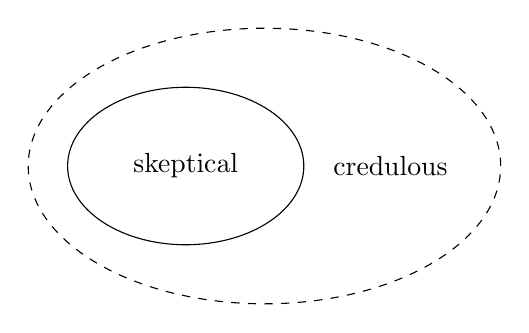
\begin{tikzpicture}
    \tikzstyle{every node}=[font=\normalsize]

    \draw[dashed]  (4,9.25) ellipse (3cm and 1.75cm);
    \draw  (3,9.25) ellipse (1.5cm and 1cm);
    \node [font=\normalsize] at (3,9.25) {skeptical};
    \node [font=\normalsize] at (5.6,9.25) {credulous};
    \end{tikzpicture}
\end{figure}





The following three justification states refine this relatively rough classification aforementioned:



\begin{df}[justified/defeasible/overruled arguemnts]
    Given a semantics $\sigma$ and an AF $\mathcal{AF}$, 
    an argument $a$ is: 
    \begin{itemize}[itemsep=5pt,parsep=5pt,leftmargin=3em,topsep=5pt]
        \item 
        \textit{justified} iff $\forall E \in \mathcal{E}_\sigma (\mathcal{AF}): a \in E$; 
        \hfill (= skeptical justification)
        

        \item 
        \textit{defensible} iff $\exists E_1,E_2 \in \mathcal{E}_\sigma (\mathcal{AF}): a \in E_1, a \not\in E_2$;


        \item 
        \textit{overruled} iff $\forall E \in \mathcal{E}_\sigma(\mathcal{AF}): a \not\in E$. 
        \hfill ($a$ should be rejected)
    \end{itemize}
\end{df}


\end{comment}



% /////////////////////////////////////////////////////////////////////////////
\subsection{An overview of (extension-based) argumentation semantics}


In this subsection we  will provide an overview of some well--known argumentation semantics, 
starting from the very basic notion of ``na\"{i}ve semantics'' \cite[\S~3.2]{Bar.Cam.Gia2018} and then 
discussing Dung's original concepts of \textit{complete}, \textit{stable}, \textit{preferred} and \textit{grounded} semantics \cite{Dun1995}.
% , 
% as well as the subsequently introduced \textit{ideal} [Dung et al., 2007], \textit{semi-stable} [Verheij, 1996; Caminada, 2006b] and \textit{eager} [Caminada, 2007b] semantics. 


% In this subsection, 
% we will examine several well-known extension-based argumentation semantics proposed in the literature. 
% 
% It is possible to distinguish between:
% \begin{itemize}[itemsep=5pt,parsep=5pt,leftmargin=2em,topsep=5pt]
%     \item four classical semantics stem from Dung's originally  seminal paper \cite{Dun1995}, 
%     namely (1) \textit{complete}, (2) \textit{grounded}, (3) \textit{stable} and (4) \textit{preferred} semantics;


%     \item 
%     subsequent proposals introduced by various authors in the literature, 
%     including \textit{stage}, \textit{semi-stable}, \textit{ideal}, $CF2$ and \textit{prudent} semantics, 
%     those semantics often overcome some limitation or improve some undesired behavior of Dung's original approach;

%     \item 
%     but in what follows, 
%     we start from a very na\"{i}ve one, 
%     called \textit{na\"{i}ve} semantics \cite[\S~3.2]{Bar.Cam.Gia2018}.
% \end{itemize} 




\begin{remark}
    In the literature, 
    \textit{admissibility} and \textit{conflict--freeness} mentioned in \S~\ref{subsec: abstract-argumentation-frameworks} are sometimes viewed as semantics, and sometimes as properties.
    We choose to treat them as properties in this note.
\end{remark}




\begin{df}[Extension--based semantics]
\label{def: extension-semantics}
    An \textit{extension--base semantics} (\textit{semantics}, for short) $\sigma$ associates with any argumentation framework $AF = (Arg,\att)$ is a subset of $\wp(Arg)$, 
    denoted as {\color{purple} $\sigma(AF)$}. 
    %    
    The elements in $\sigma(AF)$ are called \textit{extensions} (under semantics $\sigma$) \zh{外延}. 


    Let $\mathcal{D}^\sigma$ be the class of AFs where a semantic $\sigma$ is defined, 
    that is, 
    \[
        {\color{purple} \mathcal{D}^\sigma}
            = 
        \{AF \mid \sigma(AF)\not=\emptyset\}.
    \]
    % 
    A semantics $\sigma$ is called \textit{universally defined} if $\mathcal{D}^\sigma$ includes all AFs.
    % 
    If for any $AF \in \mathcal{D}^\sigma$ we have that $|\sigma(AF)| = 1$, 
    i.e. the semantics $\sigma$ always prescribes exactly one extension, 
    then $\sigma$ is said to belong to the \textit{unique--status approach}, 
    it is said to belong to the \textit{multiple--status approach}, 
    otherwise. 
    \zh{基于外延的语义}
\end{df}



% /////////////////////////////////////
\subsubsection{Na\"{i}ve Semantics}


\textit{Na\"{i}ve semantics} (denoted as {\color{purple} $\mathcal{N}\!\mathcal{A}$}) corresponds to selecting as many arguments as possible, 
provided that there are no conflicts among them.  
% 
It is a sort of greedy strategy, 
driven by the only criterion of avoiding conflicts. 
% 
Formally it corresponds to requiring conflict--freeness together with a maximality property.




\begin{df}[Na\"{i}ve extensions]
    Let $(Arg,\att)$ be an AF. 
    % 
    A set $X \subseteq Arg$ is called a \textit{na\"{i}ve extension} iff 
    $X$ is a maximal conflict--free set.
\end{df}


\begin{example}
    \qquad
    \begin{center}
    \renewcommand{\arraystretch}{1.3}
    \begin{tabular}{c||c}
        \hline
        $AF$ & 
        na\"{i}ve  extensions $ \mathcal{N}\!\mathcal{A}(AF)$ \\ 
        \hline
    
    
        \begin{tikzcd}
            a & b & c & d
            \arrow[from=1-1, to=1-2]
            \arrow[from=1-2, to=1-3]
            \arrow[curve={height=-10pt}, from=1-3, to=1-4]
            \arrow[curve={height=-10pt}, from=1-4, to=1-3]
        \end{tikzcd} & 
        $\{ a,c \}, \{ a,d \}, \{b,d\}$  \\
    
        \hline 
    
        \begin{tikzcd}
            a & c \\
            b & d
            \arrow[from=1-1, to=1-2]
            \arrow[curve={height=-6pt}, from=1-1, to=2-1]
            \arrow[from=1-2, to=2-2]
            \arrow[curve={height=-6pt}, from=2-1, to=1-1]
            \arrow[from=2-1, to=1-2]
        \end{tikzcd}  &
        $\{a,d\}, \{b,d\},\{c\}$ \\
    
        \hline 
    
        \begin{tikzcd}
            a & b \\
            & c
            \arrow[curve={height=-6pt}, from=1-1, to=1-2]
            \arrow[curve={height=-6pt}, from=1-2, to=2-2]
            \arrow[curve={height=-12pt}, from=2-2, to=1-1]
        \end{tikzcd} & 
        $\{a\}, \{b\}, \{c\}$ \\
        \hline
    \end{tabular}
    \end{center}
\end{example}

  




% % /////////////////////////////////////
\subsubsection[Complete Semantics]{Complete Semantics \zh{完全语义}}

% $X$ 防御的所有论证都在 $X$ 中

\textit{Complete semantics} (denoted as {\color{purple} $\mathcal{CO}$}) can be regarded as a strengthening of the basic 
requirements enforced by the idea of admissibility, 
it lies at the heart of all Dung's semantics (see Fig.~\ref{fig: relations among extension notions}).


A complete extension is a conflict--free set which includes precisely those arguments it defends. 
That is, 
if an argument is defended by the set it should be in the set, 
and if an argument is not defended by the set, it should not be in the set.


\begin{df}[Complete extensions]
    Let $AF=(Arg,\att)$ be an AF. 
    %
    A set $X \subseteq Arg$ is called a \textit{complete extension} iff $X$ is conflict--free and $X = C_{AF}(X)$. 
\end{df}


Technically this means that a complete extension is a \textit{conflict--free fixed point} of the characteristic function.
% 
It is clear that every complete extension is an admissible set, 
but the reverse does not hold in general. 
\zh{无冲突不动点}
\\ 
``Intuitively, 
the notion of complete extension captures the kind of confident relational agent who believe in every thing he can defend''\cite{Dun1995}.



\begin{prop} Let $AF = (Arg,\att)$ be any AF.
    \begin{itemize}[itemsep=5pt,parsep=5pt,leftmargin=3em,topsep=5pt]
        \item $\mathcal{CO}(AF) \not= \emptyset$, 
        that is, 
        complete semantics is universally defined (see Definition~\ref{def: extension-semantics}).


        \item 
        $\emptyset \in \mathcal{CO}(AF)$ iff $\mathcal{NI}(AF) = \emptyset$, 
        where $\mathcal{NI}(AF) \coloneqq \{a \mid a^- = \emptyset\}$.

        
        \item 
        $\forall E \in \mathcal{CO}(AF): \mathcal{NI}(AF) \subseteq E$.
    \end{itemize}
\end{prop}






% complete extensions
\begin{example} \qquad

    \begin{center}
    \renewcommand{\arraystretch}{3}
    \begin{tabular}{c||c}
    \hline
        $AF$ & 
        complete extensions $\mathcal{E}_\mathcal{CO}(AF)$ \\ 
        \hline
    
    
        \begin{tikzcd}
            a & b & c & d
            \arrow[from=1-1, to=1-2]
            \arrow[from=1-2, to=1-3]
            \arrow[curve={height=-10pt}, from=1-3, to=1-4]
            \arrow[curve={height=-10pt}, from=1-4, to=1-3]
        \end{tikzcd} & 
        $\{a\}, \{a,d\}, \{a,c\}$  \\
    
        \hline 
    
        \begin{tikzcd}
            a & c \\
            b & d
            \arrow[from=1-1, to=1-2]
            \arrow[curve={height=-6pt}, from=1-1, to=2-1]
            \arrow[from=1-2, to=2-2]
            \arrow[curve={height=-6pt}, from=2-1, to=1-1]
            \arrow[from=2-1, to=1-2]
        \end{tikzcd}  &
        $\emptyset, \{a,d\}, \{b,d\}$ \\
    
        \hline 
    
        \begin{tikzcd}
            a & b \\
            & c
            \arrow[curve={height=-6pt}, from=1-1, to=1-2]
            \arrow[curve={height=-6pt}, from=1-2, to=2-2]
            \arrow[curve={height=-12pt}, from=2-2, to=1-1]
        \end{tikzcd} & 
        $\emptyset$ \\
        \hline
    \end{tabular}
    \end{center}
\end{example}








% % /////////////////////////////////////
\subsubsection[Grounded Semantics]{Grounded Semantics \zh{基语义}}

% 满足怀疑的评价标准(最小的完全外延)

To accept only the arguments that one cannot avoid accepting, 
to reject only the arguments that one cannot avoid rejecting, 
and abstaining as much as possible.
% 
This gives rise to the {\color{teal} most skeptical semantics} among those based on complete extensions, 
namely the 
\textit{grounded semantics} (denoted as {\color{purple} $\mathcal{GR}$}).




\begin{df}[The grounded extension]
    Let $AF=(Arg,\att)$ be an AF.
    % 
    The \textit{grounded extension} of $AF$ is a minimal conflict--free fixed point of the characteristic function.
\end{df}


Notice that the {\color{teal} uniqueness} of the grounded extension. 
Since the characteristic function $C_{AF}$ is monotonic, 
it follows from the Knaster-Tarski Theorem that $C_{AF}$ has a unique smallest fixed point, 
it can then be proved that this fixed point is also conflict--free.



\begin{prop}
    For any AF $AF=(Arg,\att)$, 
    the following statements are equivalent:
    \begin{enumerate}[itemsep=5pt,parsep=5pt,leftmargin=3em,topsep=5pt,label=(\arabic*)] 
        \item $X$ is a minimal conflict--free fixed point of $C_{AF}$.
        
        \item $X$ is the smallest fixed point of $C_{AF}$.
    \end{enumerate} 
\end{prop}



It follows that:
\begin{itemize}[itemsep=5pt,parsep=5pt,leftmargin=3em,topsep=5pt]
    \item the grounded extension is unique 
    (i.e. grounded semantics belongs to the unique-status approach);


    \item the grounded extension is the least complete extension, 
    in particular it is included in any complete extension.
\end{itemize}




The grounded extension of an argumentation framework $AF$ will be denoted as {\color{purple} $GR(AF)$}.
% 
By definition,
the grounded extension coincides with the intersection of all complete extensions, 
that is 
\[
    GR(AF) = \bigcap \mathcal{CO} (AF).
\]
Hence, 
a unique grounded extension always exists, 
although it may be the empty set. 
% 
% It contains all the arguments which are not defeated, 
% as well as the arguments which are defended directly or indirectly by non-defeated arguments.



\begin{prop}
    If there are no initial arguments in an AF, 
    then the grounded extension is the empty set. 
    % 
    That is, 
    $\mathcal{IN}(AF) = \emptyset \Rightarrow GR(AF)=\emptyset$.
\end{prop}


\begin{example}[Grounded extension] \qquad

    \begin{center}
    \renewcommand{\arraystretch}{3}
    \begin{tabular}{c||c}
    \hline
        $AF$ & 
        grounded extensions $\mathcal{GR}(AF)$ \\ 
        \hline
    
    
        \begin{tikzcd}
            a & b & c & d
            \arrow[from=1-1, to=1-2]
            \arrow[from=1-2, to=1-3]
            \arrow[curve={height=-10pt}, from=1-3, to=1-4]
            \arrow[curve={height=-10pt}, from=1-4, to=1-3]
        \end{tikzcd} & 
        $\{a\}$  \\
    
        \hline 
    
        \begin{tikzcd}
            a & c \\
            b & d
            \arrow[from=1-1, to=1-2]
            \arrow[curve={height=-6pt}, from=1-1, to=2-1]
            \arrow[from=1-2, to=2-2]
            \arrow[curve={height=-6pt}, from=2-1, to=1-1]
            \arrow[from=2-1, to=1-2]
        \end{tikzcd}  &
        $\emptyset$ \\
    
        \hline 
    
        \begin{tikzcd}
            a & b \\
            & c
            \arrow[curve={height=-6pt}, from=1-1, to=1-2]
            \arrow[curve={height=-6pt}, from=1-2, to=2-2]
            \arrow[curve={height=-12pt}, from=2-2, to=1-1]
        \end{tikzcd} & 
        $\emptyset$ \\
        \hline
    \end{tabular}
    \end{center}
\end{example}




% % /////////////////////////////////////
\subsubsection[Preferred Semantics]{Preferred Semantics \zh{优先语义}}

% 满足轻信的评价标准(极大的完全外延)

The idea of maximizing accepted arguments is expressed by \textit{preferred semantics} ({\color{purple} $\mathcal{PR}$}, in symbol).


\begin{df}[Preferred extensions]
    Let $AF=(Arg,\att)$ be an AF. 
    %
    A \todo{优先外延} \textit{preferred extension} is a maximal (w.r.t. $\subseteq$) admissible set of $AF$. 
\end{df}



Every argumentation framework possesses at least one preferred extension.
Hence, 
preferred extension semantics is always defined for any argumentation framework. 
% 
Relationships of preferred extensions with other semantics notions have been analyzed in Dung's \cite{Dun1995}. 
%
Preferred extensions can for instance equivalently be characterized as maximal complete extensions.


\begin{prop}
    Let $AF=(Arg,\att)$ be an AF and $X \subseteq Arg$. 
    The following two statements are equivalent:
    \begin{enumerate}[itemsep=5pt,parsep=5pt,leftmargin=3em,topsep=5pt,label=(\arabic*)] 
        \item $X$ is a maximal admissible set of $AF$.
        
        \item $X$ is a maximal complete extension of $AF$.
    \end{enumerate}
\end{prop}


This in particular implies that the grounded extension is included in any preferred extension, 
as it is in any complete extension.


Preferred semantics has often been regarded as the most satisfactory semantics in the context of Dung's framework.



\begin{example}[Preferred extensions] \qquad

    \begin{center}
    \renewcommand{\arraystretch}{3}
    \begin{tabular}{c||c}
    \hline
        $AF$ & 
        preferred extensions $\mathcal{PR}(AF)$ \\ 
        \hline
    
        \begin{tikzcd}
            a & b & c & d
            \arrow[from=1-1, to=1-2]
            \arrow[from=1-2, to=1-3]
            \arrow[curve={height=-10pt}, from=1-3, to=1-4]
            \arrow[curve={height=-10pt}, from=1-4, to=1-3]
        \end{tikzcd} & 
        $\{a,d\}, \{a,c\}$  \\
    
        \hline 
    
        \begin{tikzcd}
            a & c \\
            b & d
            \arrow[from=1-1, to=1-2]
            \arrow[curve={height=-6pt}, from=1-1, to=2-1]
            \arrow[from=1-2, to=2-2]
            \arrow[curve={height=-6pt}, from=2-1, to=1-1]
            \arrow[from=2-1, to=1-2]
        \end{tikzcd}  &
        $\{a,d\}, \{b,d\}$ \\
    
        \hline 
    
        \begin{tikzcd}
            a & b \\
            & c
            \arrow[curve={height=-6pt}, from=1-1, to=1-2]
            \arrow[curve={height=-6pt}, from=1-2, to=2-2]
            \arrow[curve={height=-12pt}, from=2-2, to=1-1]
        \end{tikzcd} & 
        $\emptyset$ \\
        \hline
    \end{tabular}
    \end{center}
\end{example}




% % /////////////////////////////////////
\subsubsection[Stable Sematnics]{Stable Semantics \zh{稳定语义}}


\textit{Stable semantics} (denoted as {\color{purple}$\mathcal{ST}$}) relies on a very simple intuition: 
an extension should be able to attack all arguments not included in it.


\begin{df}[Stable extensions]
    Let $AF=(Arg,\att)$ be an AF. 
    %
    A \textit{stable extension} \zh{稳定外延} of $AF$ is a conflict--free set $X$ such that $X \cup X^+ = Arg$. 
\end{df}


A stable extension is an admissible set.
% 
In the context of game theory, 
the notion of stable extension coincides with the notion of \textit{stable solution} of $n$-person games \cite{Dun1995}. 
% 
Every stable extension is a preferred extension, 
but not vice versa. 


\begin{prop}
    Let $AF=(Arg,\att)$ be an AF and $X \subseteq Arg$. 
    The following statements are equivalent:
    \begin{enumerate}[itemsep=5pt,parsep=5pt,leftmargin=3em,topsep=5pt,label=(\arabic*)] 
        \item $X$ is a stable extension. 
        
        \item $X$ is an admissible set s.t. $X \cup X^+ = Arg$.
        
        \item $X$ is a complete extension s.t. $X \cup X^+ = Arg$.
        
        \item $X$ is a preferred extension s.t. $X \cup X^+ = Arg$.
        
        \item $X^+ = Arg \setminus X$.
    \end{enumerate}
\end{prop}


No stable extension is empty, 
and not every argument framework has stable extensions.



\begin{example}[Stable extensions] \qquad
    \begin{center}
    \renewcommand{\arraystretch}{3}
    \begin{tabular}{c||c}
    \hline
        $AF$ & 
        stable extensions $\mathcal{ST}(AF)$ \\ 
        \hline
    
    
        \begin{tikzcd}
            a & b & c & d
            \arrow[from=1-1, to=1-2]
            \arrow[from=1-2, to=1-3]
            \arrow[curve={height=-10pt}, from=1-3, to=1-4]
            \arrow[curve={height=-10pt}, from=1-4, to=1-3]
        \end{tikzcd} & 
        $\{a,d\}, \{a,c\}$  \\
    
        \hline 
    
        \begin{tikzcd}
            a & c \\
            b & d
            \arrow[from=1-1, to=1-2]
            \arrow[curve={height=-6pt}, from=1-1, to=2-1]
            \arrow[from=1-2, to=2-2]
            \arrow[curve={height=-6pt}, from=2-1, to=1-1]
            \arrow[from=2-1, to=1-2]
        \end{tikzcd}  &
        $\{a,d\}, \{b,d\}$ \\
    
        \hline 
    
        \begin{tikzcd}
            a & b \\
            & c
            \arrow[curve={height=-6pt}, from=1-1, to=1-2]
            \arrow[curve={height=-6pt}, from=1-2, to=2-2]
            \arrow[curve={height=-12pt}, from=2-2, to=1-1]
        \end{tikzcd} & 
        $-$ \\
        \hline
    \end{tabular}
\end{center}
\end{example}



% % /////////////////////////////////////

\subsubsection{Semi-Stable Semantics (coming in soon)}




% \textit{Semi-stable semantics} ($\mathcal{SST}$) 


% \begin{df}[Semi-stable extensions]
%     Let $\mathcal{AF}=(Ar,\to)$ be an AF. 
%     A \textit{semi--stable extension} of $\mathcal{AF}$ is a complete extension $X$ where $X \cup X^+$ is maximal among all complete extensions. 
% \end{df}


% % /////////////////////////////////////
\subsubsection{Ideal and Eager Semantics (coming in soon)}

% % /////////////////////////////////////
\subsubsection{Stage Semantics (coming in soon)}

% % /////////////////////////////////////
\subsubsection{$CF2$ and stage2 Semantics (coming in soon)}


cf2: $\mathcal{CF}2$

ideal: $\mathcal{ID}$

semi--stable: $\mathcal{SST}$ 

stage: $\mathcal{STG}$

\begin{df}
    Let $AF = (Arg,\att)$ be an AF. 
    For a conflict--free set $X$, it holds that:
    \begin{itemize}[itemsep=5pt,parsep=5pt,leftmargin=3em,topsep=5pt]
        \item 
        $X \in \mathcal{ID}(AF)$ iff $X$ is $\subseteq$--maximal among $\{X' \mid X' \in ad(AF) ~\&~ X'\subseteq E \text{ for each~} E \in \mathcal{PR}(AF)\}$.

        \item 
        $X \in \mathcal{SST}(AF)$ iff $X \in ad(AF)$ and there is no $T \in ad(AF)$ with $X^\oplus \subset T^\oplus$, 
        where $X^\oplus = X^+ \cup X^-$, similar for $T^\oplus$.

        \item 
        $X \in \mathcal{STG}(AF)$ iff there is no $T \in cf(AF)$ with $X^\oplus \subset T^\oplus$.
    \end{itemize}

    Following, 
    we give the recursive definition of $CF2$ semantics.
    % 
    $X \in \mathcal{CF}2(AF)$ if
    \begin{itemize}[itemsep=5pt,parsep=5pt,leftmargin=3em,topsep=5pt]
        \item 
         $X \in \mathcal{NA}(AF)$ if $|SCC_{S_F}|=1$, and 

        \item
        $\forall S \in SCC_{S_F}$, 
        $X \cap S \in \mathcal{CF}2(AF\downharpoonright )$; 
        otherwise.
    \end{itemize}
\end{df}








% /////////////////////////////////////////////////////////////////////////////
\clearpage
\subsection{Computational problems and Complexity}

When studying computational complexity we are only interested in AFs where the arguments set $Arg$ is finite.


Given an AF $AF=(Arg,\att)$ and a semantics/property $\sigma$, 
there are several kinds of computational problems usually be considered:
\begin{enumerate}[itemsep=5pt,parsep=5pt,leftmargin=3em,topsep=5pt,label=(\arabic*)] %% or label = \alph*, \roman*
    \item 
    the \textit{verification problem}  \zh{验证问题}, 
    denoted as {\color{purple} $Var_\sigma$}: 
    deciding whether a set $X \subseteq Arg$ is a $\sigma$--extension of $AF$, 
    that is, whether $X \in \sigma(AF)$?

    \item 
    the \textit{credulous acceptance problem} \zh{轻信接受问题}, 
    denoted as {\color{purple} $Cred_\sigma$}: 
    for $a \in Arg$, 
    deciding whether $a$ is credulously accepted, 
    that is deciding whether $a$ belongs to a $\sigma$--extension of $AF$. 
    I.e., whether $a \in \bigcup \sigma(AF)$?

    Every argument that does not attack itself will be credulously accepted under the conflict--free property.

    \item 
    the \textit{skeptical acceptance problem} \zh{谨慎接受问题}, 
    denoted as {\color{purple} $Skept_\sigma$}: 
    deciding whether $a$ is skeptically  accepted, 
    that is deciding whether $a$ belongs to every $\sigma$--extension of $AF$.
    I.e.,  whether $a \in \bigcap \sigma(AF)$?
\end{enumerate}


Another task is deciding whether an AF provides any coherent conclusion.
\begin{enumerate}[itemsep=5pt,parsep=5pt,leftmargin=3em,topsep=5pt] 
    \item[(4)] 
    \textit{Existence of an extension} \zh{外延存在问题}, 
    {\color{purple} $Exists_\sigma$}: Is $\sigma(AF) \not= \emptyset$?

    \item[(5)] 
    Existence of a non--empty extension \zh{非空外延存在问题}, 
    {\color{purple} $Exists_\sigma^{-\emptyset}$}: 
    Does there exist a set $S \not=\emptyset$ such that $S \in\sigma(AF)$?
\end{enumerate}


Finally, 
we will also consider the problem of deciding whether a semantics
yields a unique extension for a given an AF:
\begin{enumerate}[itemsep=5pt,parsep=5pt,leftmargin=3em,topsep=5pt,] 
    \item[(6)]
    \textit{Uniqueness of the solution}, 
    {\color{purple} $Unique_\sigma$}, 
    Is there a unique set $X \in \sigma(AF)$, i.e., 
    is $\sigma(AF)=\{X\}$?
\end{enumerate}



Clearly, 
$CA_\tau$ and $SA_\tau$ are identical problems with $\tau \in \{\mathcal{GR},\mathcal{ID}\}$.
% 
For $\sigma \in \{\mathcal{CO,GR,PR,ST}\}$, 
the computational complexity of those problems are summarized in  table~\ref{tab: complexity} (for more detail, see \cite{Dun.Woo2009,Dvo.Dun2018}).




\begin{table}[th!]
    \centering
    \caption{Complexity of some problems}
    \label{tab: complexity}
    %%
    \renewcommand{\arraystretch}{1.5}
    \begin{tabular}{c||ccc}
    \hline

    semantics or properties & 
    $Ver_\sigma$ & $Cred_\sigma$ & $Skept_\sigma$   \\
    \hline

    $cf$ & 
    in \textsf{L} & 
    in \textsf{L} & 
    trivial \\

    $ad$ & 
    in \textsf{L} & 
    \textsf{NP--c} & 
    trivial \\

    \hline

    $\mathcal{CO}$ & 
    in \textsf{P} & 
    \textsf{NP--c} & 
    \textsf{P--c}  \\

    $\mathcal{GR}$ & 
    in \textsf{P} & 
    in \textsf{P} & 
    in \textsf{P}  \\

    $\mathcal{PR}$ & 
    \textsf{coNP--c} & 
    \textsf{NP--c} & 
    \textsf{$\prod^p_2$--c}  \\

    $\mathcal{ST}$ & 
    in \textsf{P} & 
    \textsf{NP--c} & 
    \textsf{coNP--c} \\
    
    \hline 

    $\mathcal{SST}$ (semi--stable) & 
    \textsf{coNP--c} & 
    \textsf{$\sum^p_2$--c} & 
    \textsf{$\prod^p_2$--c}  \\

    \hline
\end{tabular}

\vspace*{1em}
\parbox{10cm}{\footnotesize
Cf \cite[Table 1]{Dvo.Dun2018}
}
\end{table}





\vspace*{3em}
% One of the most common reasoning problems in argumentation concerns the skeptical and credulous acceptance of arguments, 
% by which we understand that they are accepted in all (resp. some) extensions of a given framework.


\noindent\dotfill some symbols \noindent\dotfill


$AF \vsim^c_\sigma a$ credulously accepted

$AF \vsim^s_\sigma a$ skeptically accepted

$AF \vsim^\circ_\sigma a$  where $\circ \in \{s,c\}$




% /////////////////////////////////////////////////////////////////////////////
\newpage
\newgeometry{left=1cm,right=1cm,top=2cm,bottom=2cm}
\subsection{A summary}



The grounded extension is uniquely determined and always exists \cite{Dun1995},
and not every framework is guaranteed to produce a stable extension.

It is well--known that
the set of \textbf{complete extensions} forms a {\color{teal} \textit{complete semilattice}} w.r.t. $\subseteq$, 
where $GR(AF)$ is the meet element, 
whereas the greatest elements are the preferred extensions.

\dotfill

- for any of the considered semantics $\sigma$ except stable semantics we have that $\sigma(AF) \not= \emptyset$ holds, 
i.e., these semantics always propose at least one extension.

- Grounded and ideal semantics always yield exactly one extension.

-  stable, semi-stable, and stage semantics coincide for AFs with at least one stable extension.

$\mathcal{ST} \subseteq \mathcal{STG} \subseteq \mathcal{NA} \subseteq cf$

$\mathcal{ST} \subseteq \mathcal{SST} \subseteq \mathcal{PR} \subseteq \mathcal{CO} \subseteq ad \subseteq cf$

$\mathcal{ST} \subseteq \mathcal{CF}2 \subseteq \mathcal{NA}$




% % figure
\begin{figure}[ht!]
    \vspace{1.5em}
    \centering
    \begin{tikzcd}
	& \text{$\mathcal{ST}$: stable~extension}  \\
	& \text{$\mathcal{PR}$: preferred~extension} \\
	\text{$\mathcal{GR}$: grounded~extension}^\ast  & \text{$\mathcal{CO}$: complete~extension} & \text{$\mathcal{NA}$: na\"{i}ve~extension} \\
	& \text{$ad$: admissible} \\
	& \text{$cf$: conflict-free}  \\
	\arrow[from=1-2, to=2-2]
	\arrow[curve={height=-12pt}, from=1-2, to=3-3]
	\arrow[from=2-2, to=3-2]
	\arrow[from=3-1, to=3-2]
	\arrow[from=3-2, to=4-2]
	\arrow[curve={height=-12pt}, from=3-3, to=5-2]
	\arrow[from=4-2, to=5-2]
    \end{tikzcd}
\caption{Relations among extension--based semantics}
\label{fig: relations among extension notions}
\vspace{1em}
\parbox{10cm}{\footnotesize
Note: The intuitive meaning of  arrow ``$x \longrightarrow y$'' is that  ``every $x$ is a $y$''.
% while the dashed arrow ``$x \dashrightarrow y$'' means that ``every $x$ is contained in any $y$''. 
For example, 
every stable extension is a preferred extension.
% , 
% as well as, 
% the grounded extension is included in any preferred extensions.
$^\ast$ denotes this semantics is unique status semantics.
}
\end{figure}


\vspace{1.5em}
\begin{table}[ht!]
    \centering
    \caption{A summary of the examples mentioned}
    \label{tab: example}
    \renewcommand{\arraystretch}{1.5}
    \begin{tabular}{c||ccccc}
    \hline
    AF & 
    na\"{i}ve  &
    complete & 
    grounded & 
    preferred & 
    stable \\
    \hline

    
    $\begin{tikzcd}
        a & b & c & d
        \arrow[from=1-1, to=1-2]
        \arrow[from=1-2, to=1-3]
        \arrow[curve={height=-10pt}, from=1-3, to=1-4]
        \arrow[curve={height=-10pt}, from=1-4, to=1-3]
    \end{tikzcd}$  & 
    $\begin{matrix} 
        \{a,c\}  \\
        \{a,d\}  \\
        \{b,d\}
    \end{matrix}$ & 
    $\begin{matrix} 
        \{a\}  \\
        \{a,c\}  \\
        \{a,d\}  
    \end{matrix}$  & 
    $\{a\}$  & 
    $\begin{matrix}
        \{a,c\} \\
        \{a,d\} 
    \end{matrix}$  & 
    $\begin{matrix}
        \{a,c\} \\
        \{a,d\} 
    \end{matrix}$  \\    
    [4ex]
    \hline 



    \begin{tikzcd}
        a & c \\
        b & d
        \arrow[from=1-1, to=1-2]
        \arrow[curve={height=-6pt}, from=1-1, to=2-1]
        \arrow[from=1-2, to=2-2]
        \arrow[curve={height=-6pt}, from=2-1, to=1-1]
        \arrow[from=2-1, to=1-2]
    \end{tikzcd} &  
    $\begin{matrix}
        \{a,d\} \\
        \{b,d\} \\
        \{c\}
    \end{matrix}$   & 
    $\begin{matrix}
        \emptyset \\
        \{a,d\} \\
        \{b,d\}
    \end{matrix}$  & 
    $\emptyset$   &  
    $\begin{matrix}
        \{a,d\} \\
        \{b,d\} 
    \end{matrix}$  &
    $\begin{matrix}
        \{a,d\} \\
        \{b,d\}
    \end{matrix}$  \\
    [4ex]
    \hline
   


    \begin{tikzcd}
        a & b \\
        & c
        \arrow[curve={height=-6pt}, from=1-1, to=1-2]
        \arrow[curve={height=-6pt}, from=1-2, to=2-2]
        \arrow[curve={height=-12pt}, from=2-2, to=1-1]
    \end{tikzcd} & 
    $\begin{matrix}
        \{a\} \\
        \{b\} \\
        \{c\}
    \end{matrix}$  & 
    $\emptyset$  & 
    $\emptyset$  & 
    $\emptyset$  & 
    $-$  \\
    [4ex]
    \hline
\end{tabular}
\end{table}


\begin{table}[ht!]
    \centering
    \caption{Some basic concepts}
    \label{tab: basic notions of AAT}
    $AF = (Arg,\att)$ is an AF and $X\cup\{a,b\} \subseteq Arg$.
    \vspace{1em}

    \renewcommand{\arraystretch}{1.3}
    \begin{tabular}{l||lll}
    % Let $\mathcal{A} = (A,\to)$ be an abstract argumentation framework \\
    \hline
    \multicolumn{1}{c}{Notions}  & 
    \multicolumn{1}{c}{Definition or equivalent descriptions} \\
    \hline

    \multirow{2}{*}{$a \att b$}   &
    $a$ attacks/defeats $b$  \\ 
    &  $a$ is an attacker/counterargument of $b$   \\

    \hdashline

    $X \att a$ \qquad   & 
    $X$ attacks $a$: $\exists b \in X: b \att a$  \\

    
    
    $a^-$ &  
    $a^- = \{b \in Arg \mid b \att a\}$  \\

    $a^+$ &  
    $a^+ = \{b \in Arg \mid a \att b\}$  \\

    $X^-$ &  
    $X^- = \{b \in Arg \mid \exists a \in X: b \att a\} = \bigcup_{a\in X} a^- $\\

    $X^+$ & 
    $X^+ = \{b \in Arg \mid \exists a \in X: a \att b\} = \bigcup_{a\in X} a^+$ \\

    $\mathcal{IN}(AF)$: the set of initial arguments &
    $\mathcal{IN}(AF) = \{a\in Arg \mid a^- = \emptyset\}$    \\

    $X$ defends $a$  / $a$ is admissible w.r.t. $X$ & 
    $\forall b: b \att a \Rightarrow X \att b$ 
    \hfill
    [$X$ defends all initial arguments] \\

    


    \hdashline

    \multirow{3}*{
    $C_{AF}$: the characteristic function}  
    & 
    % $C_\mathcal{AF} \colon \wp(Ar) \att \wp(Ar)$ s.t. 
    $C_{AF} (X) = \{a \mid X \text{~defends~} a \}$   \\
    &  $C_{AF}{X} = (X^+)^+$  \\
    & [$\emptyset$ is a fixed point if $\mathcal{IN}(AF)=\emptyset$]  \\

    \hdashline


    \multirow{3}{*}{$cf(AF) \ni X$ is conflict--free} & 
    $\not\exists a,b \in X: a \att b$ 
    \hfill
    [$\emptyset$ is conflict--free]  \\
    & 
    $\not\exists a,b \in X: a \in b^-$  \\ 
    & 
    $X \cap X^+ = \emptyset$    \\
    % $\forall a,b \in X: a \not\att b$  \\


    \hdashline


    $ad(AF) \ni X$ is admissible & 
    $X$ is conflict--free and $X \subseteq C_\mathcal{AF} (X)$  
    \hfill
    [$\emptyset$ is admissible] \\

    
    \hline
    \multicolumn{2}{c}{\textsc{Semantics}} \\
    \hline

    $\mathcal{N}\!\mathcal{A}(AF) \ni X$ is a \textit{na\"{i}ve extension} & 
    $X$ is a maximal conflict--free set  \\
    \hdashline 

    
    \multirow{2}{*}{$\mathcal{CO}(AF) \ni X$ is a \textit{complete extension}} &  
    $X$ is a conflict--free  and $C_{AF}(X)=X$  \\
    & conflict--free fixed point \\
    \hdashline


    \multirow{3}{*}{$\mathcal{GR}(AF) \ni X$ is the \textit{grounded extension} 
    } & 
    $X$ is the least fixed point of $C_{AF}$  \\
    & $X$ is the minimal complete extension  \\
    & $X = GR(AF) = \bigcap \mathcal{CO}(AF)$  \\

    
    \hdashline

    
    \multirow{2}{*}{$\mathcal{PR}(AF) \ni X$ is a \textit{preferred extension}  
    } & 
    $X$ is a maximal admissible set  \\
    & $X$ is a maximal complete extension  \\ 
    \hdashline

    
    \multirow{7}{*}{$\mathcal{ST}(AF) \ni X$ is a \textit{stable extension}
    } & 
    $X$ is conflict--free and $X \cup X^+ = Arg$  \\
    & $X^+ = Arg \setminus X$    \\
    & $X$ is a preferred extension and $X \cup X^+ = Ar$  \\
    & $X$ is a complete extension and $X \cup X^+ = Ar$  \\
    & $X$ is admissible and $X \cup X^+ = Ar$  \\ 
    & $X = \{a \in Ar \mid X \not\att a\}$  \\
    & $X$ is conflict--free and attacks each argument that is not in $X$  \\
    \hline
    \end{tabular}

    % \vspace{1em}
    % NB: all the key argumentation-theoretic notions can be defined in terms of the characteristic function.
\end{table}



\restoregeometry
% /////////////////////////////////////////////////////////////////////////////